\chapter{Subgradien}\label{d90-hab:ch:subgradien}

% segment-id: d90.hab.v1.ch03.seg0001
Ingat kembali definisi turunan (Fréchet).

Sepanjang bab ini, \(X\) dan \(Y\) menyatakan ruang bernorma real; apabila gradien digunakan, \(X\) merupakan ruang Hilbert. Setiap kali \(V\) atau \(W\) muncul, keduanya menyatakan ruang bernorma real berdimensi hingga. Pada pasangan dual, argumen pertama selalu fungsional dan argumen kedua selalu vektor.

\begin{defn}[Turunan Fréchet]
    Misalkan $f:X\rightarrow Y$. Fungsi $f$ dikatakan terdiferensialkan (dalam arti Fréchet) di $x\in X$ apabila terdapat pemetaan linear kontinu $A:X\rightarrow Y$ sedemikian sehingga
    \begin{equation}
        \lim_{\|h\|\rightarrow 0}\frac{\| f(x+h) - f(x)  -Ah\|}{\|h\|}= 0.
    \end{equation}
    Kita menuliskan $A=Df(x)$.
\end{defn}

\begin{defn}[Gradien]
    Misalkan $f:X\rightarrow \R$ terdiferensialkan dan $X$ merupakan ruang Hilbert. Gradien $f$ di titik $x$, yang dilambangkan dengan $\nabla f(x)$, adalah unsur tunggal di $X$ sedemikian sehingga
    \begin{equation}
        Df(x)h =  \inner{\nabla f(x)}{h}, \quad h\in X.
    \end{equation}
\end{defn}

Keberadaan dan ketunggalan gradien merupakan akibat langsung dari teorema representasi Riesz, sebab $Df(x)\in X^*$ apabila $f$ bernilai real. Perhatikan pula bahwa \textbf{gradien bergantung pada hasil kali dalam yang dipilih}.

Walaupun definisi umum di atas mungkin tampak agak abstrak, gradien yang kita temui biasanya cukup sederhana. Secara khusus, apabila $X=\R^d$ dilengkapi dengan hasil kali dalam Euklides baku, maka
\begin{equation}
    \nabla f(x) = Df(x)^T,
\end{equation}
\ie, gradien hanyalah transpos dari turunannya.

% segment-id: d90.hab.v1.ch03.seg0002
Turunan dapat ditafsirkan sebagai hampiran linear terbaik terhadap fungsi di suatu titik, yakni
\begin{equation}
    f(y) = f(x) + Df(x)(y-x) + o(\|y-x\|),
\end{equation}
dengan $o$ kecil menyatakan suatu suku yang meluruh \emph{lebih cepat daripada laju linear}. Kebanyakan metode optimisasi dapat ditafsirkan sebagai proses berulang untuk meminimumkan hampiran fungsi yang lebih mudah. Akan tetapi, banyak fungsi penting tidak memiliki gradien dalam pengertian di atas. Sebagai contoh, kita mungkin ingin menyelesaikan persoalan
\begin{equation}
    \min\limits_x \frac{1}{2}\|Ax-b\|^2_2 + \lambda\|K x\|_1,
\end{equation}
dengan $A$ dan $K$ linear. Persoalan komposit semacam ini sangat umum dalam pengolahan citra.
Karena itu, kita dapat bertanya apakah terdapat gagasan hampiran linear yang lebih umum tetapi memiliki sifat serupa dengan gradien. Definisi berikut menjawab pertanyaan ini secara positif.

\begin{defn}[Subdiferensial]
    Misalkan $f:X\rightarrow(-\infty,\infty]$ dan $x\in\dom(f)$. Kita menyebut $g\in X^*$ sebagai \emph{subgradien} $f$ di $x$ apabila
    \begin{equation}
        f(x) + \langle g, y-x\rangle\leq f(y), \quad \forall y\in X.
    \end{equation}
    Subdiferensial $\partial f(x)$ di $x$ adalah himpunan semua subgradien di $x$, yakni
    \begin{equation}
        \partial f(x) =\{ g\in X^*\;|\; f(x) + \langle g, y-x\rangle\leq f(y), \quad \forall y\in X \}.
    \end{equation}
    Untuk $x\notin\dom(f)$, kita menetapkan $\partial f(x)=\emptyset$.
\end{defn}

Jadi, subdiferensial dapat saja kosong; menurut konvensi di atas, subdiferensial kosong di setiap titik $x\in X$ dengan $f(x)=\infty$.

% segment-id: d90.hab.v1.ch03.seg0003
\Needspace{0.62\textheight}
\begin{example}\
    \begin{enumerate}
        \item Norma: Misalkan $f = \norm{\cdot}$. Maka
			\[
				\partial f(0) = \overline{B}_{\|\cdot\|_*, 1}(0),
			\]
            yaitu bola satuan untuk norma dual. Ingat bahwa norma dual $\|\cdot\|_*$ didefinisikan oleh
            \[
                \|y\|_* = \sup_{\|x\|\leq 1} |\langle y,x\rangle|.
            \]
			Sebagai contoh, apabila $f = \|\cdot\|_1$ pada $\R^n$, maka
			\[
				\partial f(0) = \overline{B}_{\|\cdot\|_\infty,1}(0) = [-1,1]^n.
			\]
        \item Untuk suatu himpunan tak kosong $S \subseteq X$ dan titik $x \in S$, tinjau fungsi indikator $\delta_S$. Subdiferensialnya adalah
			\[
				\partial\delta_S(x)=\left\{y\in X^\ast:\inner{y}{z-x}\leq 0,\;\forall z\in S\right\}\eqqcolon N_S(x),
			\]
			yang disebut \emph{kerucut normal} $S$ di $x$.
			Subdiferensial fungsi indikator dari bola satuan adalah
			\[
				N_{\overline{B}_{\|\cdot\|, 1}(0)}(x)=
				\begin{cases}
					\{y\in X^\ast\mid\|y\|_*\leq \inner{y}{x}\}&\text{jika }\norm{x}\leq 1,\\
					\emptyset&\text{jika }\norm{x}>1.
				\end{cases}
            \]
    \end{enumerate}
\end{example}

% segment-id: d90.hab.v1.ch03.seg0004
Kita perlu memastikan bahwa subdiferensial benar-benar memperumum gradien biasa.

\begin{lemma}
    Misalkan $f:X\rightarrow \R$ konveks dan terdiferensialkan di $x\in \dom(f)^\circ$, dengan $X$ ruang Hilbert. Maka $\partial f(x) = \{\nabla f(x)\}$.
\end{lemma}
\begin{proof}
    Kita perlu menunjukkan (i) $\nabla f(x)\in \partial f(x)$ dan (ii) jika $g\in\partial f(x)$, maka $g=\nabla f(x)$. Bagian (i) langsung mengikuti karakterisasi orde pertama untuk fungsi konveks terdiferensialkan, yang memberikan
    \begin{equation}
        f(x) + \inner{\nabla f(x)}{y-x}\leq f(y),\quad y\in X,
    \end{equation}
    sehingga $\nabla f(x)\in\partial f(x)$. Untuk (ii), menurut definisi subgradien, bagi setiap $g\in\partial f(x)$, $h\in X$, dan $t>0$ yang cukup kecil sehingga $x+th\in\dom(f)$, berlaku
    \begin{equation}
        \inner{g}{h}\leq \frac{f(x+th)-f(x)}{t}.
    \end{equation}
    Dengan mengambil limit $t\rightarrow 0$, diperoleh $\inner{g}{h}\leq \inner{\nabla f(x)}{h}$. Menerapkan ketaksamaan yang sama pada $-h$ memberikan ketaksamaan sebaliknya. Karena itu $\inner{g}{h}= \inner{\nabla f(x)}{h}$ untuk setiap $h$, sehingga $g=\nabla f(x)$.
\end{proof}
Dalam dimensi hingga, kebalikannya juga berlaku bagi fungsi konveks yang hingga pada suatu lingkungan titik $x$: jika subdiferensial di $x$ hanya terdiri atas satu unsur, maka $f$ terdiferensialkan di $x$ dan $\partial f(x) = \{\nabla f(x)\}$.

\begin{figure}
    \centering
    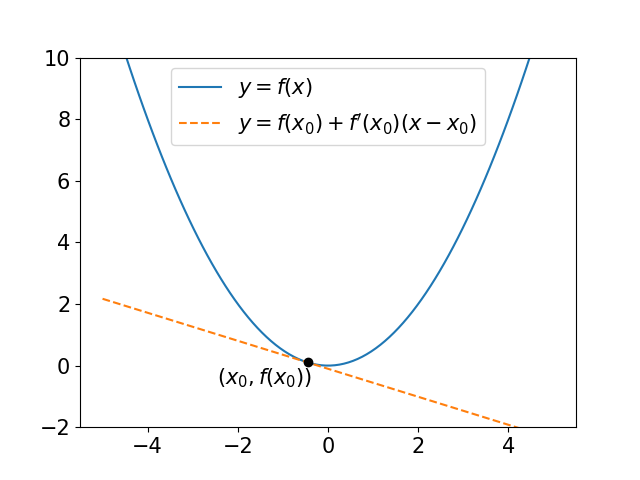
\includegraphics[scale=0.4]{figures/gradient}
    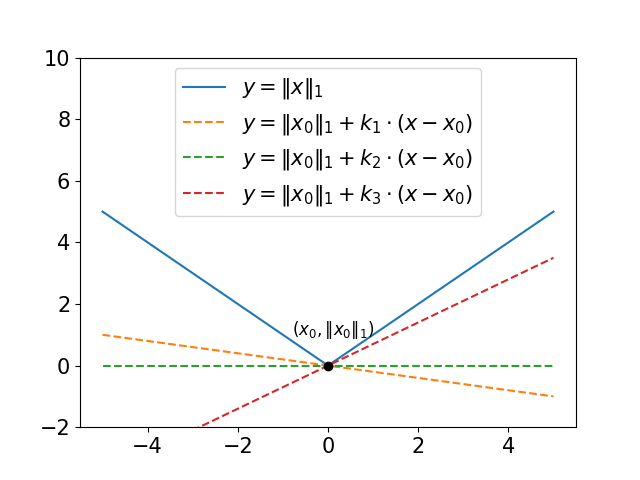
\includegraphics[scale=0.4]{figures/subgradient}
    \caption{Kiri: gradien sebagai kemiringan garis singgung. Kanan: sebuah subgradien sebagai kemiringan garis pendukung.}
\end{figure}

\noindent\textbf{Deskripsi gambar.} Panel kiri memperlihatkan parabola halus dan satu garis singgung putus-putus pada titik yang ditandai. Panel kanan memperlihatkan grafik berbentuk V untuk norma satu dimensi dan tiga garis pendukung dengan kemiringan berbeda yang semuanya melalui titik sudut yang ditandai. Label matematis pada kedua figur dipertahankan persis dari aset sumber.

\Needspace{0.50\textheight}
\begin{example}\
    \begin{enumerate}
        \item Untuk $f(x)=\|x\|_2$, diperoleh
        \[
            \partial f(x)
            = \begin{cases}
                \{\frac{x}{\|x\|_2}\}\quad& x\neq 0,\\
                \overline{B}_{\|\cdot\|_2,1}(0)\quad&\text{selain itu}.
            \end{cases}
        \]
        \item Khususnya, untuk $d=1$ dan $f(x)=|x|$, diperoleh
        \[
            \partial f(x)
            = \begin{cases}
                \{\sign(x)\}\quad& x\neq 0,\\
                [-1,1]\quad&\text{selain itu}.
            \end{cases}
        \]
    \end{enumerate}
\end{example}

% segment-id: d90.hab.v1.ch03.seg0005
\begin{lemma}
    Jika domain $f:X\rightarrow(-\infty,\infty]$ konveks dan subdiferensialnya tak kosong di setiap titik dalam domain, maka $f$ konveks.
\end{lemma}
\begin{proof}
    Misalkan $x,y\in \dom f$, $\lambda\in (0,1)$, dan $g\in \partial f(x+\lambda (y-x))$.
    Menurut definisi subdiferensial,
    \begin{gather}
        f(x+\lambda(y-x)) + \langle g, x - (x+\lambda(y-x))\rangle \leq f(x),\\
        f(x+\lambda(y-x)) + \langle g, y - (x+\lambda(y-x))\rangle \leq f(y),
    \end{gather}
    atau, setara dengan itu,
    \begin{gather}
        f(x+\lambda(y-x)) + \langle g, -\lambda(y-x)\rangle \leq f(x),\\
        f(x+\lambda(y-x)) + \langle g, (1-\lambda)(y - x) \rangle \leq f(y).
    \end{gather}
    Dengan membagi ketaksamaan pertama oleh $\lambda$, membagi yang kedua oleh $1-\lambda$, lalu menjumlahkannya, diperoleh
    \begin{equation}
        \begin{aligned}
            \frac{1}{\lambda} f(x+\lambda(y-x)) + \frac{1}{1-\lambda} f(x+\lambda(y-x))\leq \frac{1}{\lambda} f(x) + \frac{1}{1-\lambda} f(y).
        \end{aligned}
    \end{equation}
    Mengalikan dengan $\lambda (1-\lambda)$ menghasilkan
    \begin{equation}
        \begin{aligned}
            f(x+\lambda(y-x)) \leq (1-\lambda) f(x) + \lambda f(y),
        \end{aligned}
    \end{equation}
    sebagaimana yang diperlukan.
\end{proof}

% segment-id: d90.hab.v1.ch03.seg0006
Seperti disebutkan di atas, subdiferensial dapat kosong. Namun, bagi fungsi konveks berdimensi hingga kita mempunyai jaminan berikut.

Fungsi bernilai real diperluas disebut \emph{sejati (proper)} apabila domain efektifnya tidak kosong dan fungsi itu tidak pernah bernilai minus tak hingga.

\begin{theorem}\label{convexity:thm:nonempty_subgrad}
    Misalkan $X$ ruang bernorma real berdimensi hingga dan $f:X\rightarrow\overline{\R}$ sejati dan konveks. Maka $\partial f(x)\neq \emptyset$ untuk setiap $x\in \dom(f)^\circ$.
\end{theorem}
Sebelum membuktikan hasil ini, kita memerlukan beberapa persiapan.

\begin{lemma}
    Interior suatu himpunan konveks adalah konveks.
\end{lemma}
\begin{proof}
    Misalkan $C$ konveks. Jika $C^\circ=\emptyset$, tidak ada yang perlu dibuktikan; jadi anggap $C^\circ\neq \emptyset$.
    Ambil $x,y\in C^\circ$ dan $\lambda\in (0,1)$. Kita perlu menunjukkan bahwa $x_\lambda\coloneqq\lambda x + (1-\lambda)y\in C^\circ$.
    Terdapat $\epsilon>0$ sedemikian sehingga $B_\epsilon(x),B_\epsilon(y)\subset C^\circ$. Sekarang ambil $z\in B_{\epsilon}(x_\lambda)$. Dengan demikian, $z=x_\lambda + h$ untuk suatu $\|h\|<\epsilon$. Kita dapat menuliskan
    \begin{equation}
        z = \lambda x + (1-\lambda)y + h = \lambda (x+h) + (1-\lambda)(y + h).
    \end{equation}
    Karena $x+h\in B_\epsilon(x)\subset C$ dan $y+h\in B_\epsilon(y)\subset C$, kekonveksan $C$ memberikan $z\in C$. Jadi $B_\epsilon(x_\lambda)\subset C$ dan $x_\lambda\in C^\circ$.
\end{proof}

\begin{lemma}
    Jika $C\subset\R^d,\ d\geq 1$ konveks dan $C^\circ=\emptyset$, maka terdapat hiperbidang $H$ sedemikian sehingga $C\subset H$.
\end{lemma}
\begin{proof}
    Jika \(C\) kosong, sembarang hiperbidang memenuhi kesimpulan. Selanjutnya anggap \(C\) tak kosong. Tanpa mengurangi keumuman, kita boleh menganggap $0\in C$. Jika tidak, pilih sembarang $x_0\in C$ dan tinjau $\widetilde{C}=C-x_0$; pada akhir bukti, hiperbidang yang diperoleh ditranslasikan kembali.

    Kita akan menunjukkan bahwa $C$ merupakan himpunan bagian suatu subruang berdimensi paling besar $d-1$. Andaikan sebaliknya bahwa $C$ memuat $d$ unsur yang bebas linear, yaitu terdapat $x_1,\dots,x_d\in C$ yang bebas linear. Karena $C$ konveks, selubung konveks
    \begin{equation}
        \conv((x_i)_i)=\bigg\{ \sum_{i=1}^d\lambda_i x_i\;\bigg|\; \lambda\in \Delta^d\bigg\}
    \end{equation}
    juga merupakan himpunan bagian $C$. Kita mengklaim bahwa $x_\star\coloneqq\frac{1}{2d}\sum_{i=1}^d x_i\in C^\circ$. Pertama, dari kekonveksan,
    \[
        x_\star=\frac{1}{2d}\sum_{i=1}^d x_i = \sum_{i=1}^d \frac{1}{2d} x_i + \frac{1}{2}0 \in C.
    \]
    Karena $x_i$ bebas linear, setiap $h\in\R^d$ dapat ditulis sebagai $h=\sum_i \lambda_i x_i$. Pemetaan $\lambda\mapsto h$ adalah pemetaan linear bijektif $\R^d\rightarrow\R^d$. Oleh karena itu terdapat $\epsilon>0$ sedemikian sehingga $\|h\|<\epsilon$ mengakibatkan $|\lambda_i|<\frac{1}{2d}$ untuk semua $i$. Khususnya, $\frac{1}{2d}+\lambda_i\in[0,1]$ dan $\sum_{i=1}^d(\frac{1}{2d}+\lambda_i)\in[0,1]$.
    Akibatnya, untuk setiap $\|h\|<\epsilon$,
    \begin{equation}
        x_\star+h = \sum_{i=1}^d \big(\frac{1}{2d} + \lambda_i\big) x_i + \bigg(1 - \sum_i\big(\frac{1}{2d} + \lambda_i\big) \bigg)0\in C.
    \end{equation}
    Jadi, apabila $C$ memuat $d$ unsur bebas linear, interiornya tidak mungkin kosong, sebab $B_\epsilon(x_\star)\subset C$. Ini bertentangan dengan asumsi. Maka $C$ memuat paling banyak $d-1$ unsur bebas linear. Pilih himpunan bebas linear maksimal $x_1,\dots,x_k$ di dalam \(C\); maksimalitas memberikan
    \[
        C\subset \span \{ x_i\mid i=1,\dots,k\}.
    \]
    Dimensi subruang ini kurang dari \(d\), sehingga subruang tersebut termuat dalam suatu hiperbidang. Setelah translasi balik bila diperlukan, diperoleh hiperbidang afin yang memuat himpunan semula.
\end{proof}

% segment-id: d90.hab.v1.ch03.seg0007
Dengan kedua hasil sebelumnya, kita dapat membuktikan teorema hiperbidang pendukung.
\begin{theorem}[Teorema hiperbidang pendukung]
    Misalkan $V$ ruang bernorma real berdimensi hingga, $C\subset V$ tak kosong dan konveks, serta $x_0\in \partial C = \overline{C}\setminus C^\circ$\footnote{yakni batas $C$}. Maka terdapat $a\in V^*$, $a\neq 0$, sedemikian sehingga
    \begin{equation}\label{subgradient:eq:supporting}
        \inner{a}{v}\leq \inner{a}{x_0},\quad v\in C.
    \end{equation}
\end{theorem}
\begin{proof}
    Hasil ini merupakan akibat teorema pemisahan Hahn--Banach. Kita membedakan dua kasus. Pertama, andaikan $C^\circ\neq \emptyset$. Himpunan $C^\circ$ terbuka, konveks, dan tak kosong. Teorema pemisahan Hahn--Banach dapat diterapkan pada $C^\circ$ dan $\{x_0\}$, sehingga ketaksamaan pendukung berlaku pada interior. Karena $C\subset\overline{C^\circ}$ dan fungsional pemisah kontinu, ketaksamaan itu meluas ke seluruh \(C\).

    Sebaliknya, jika $C^\circ$ kosong, lema sebelumnya memberikan hiperbidang afin $H$ yang memuat \(C\). Karena $H$ tertutup dan $x_0\in\overline C$, hiperbidang ini juga memuat titik batas tersebut. Ambil $a\in V^*$ yang tak nol dan $b\in\R$ sedemikian sehingga
    \[
        H=\{x\mid \inner{a}{x} = b\}.
    \]
    Fungsional $a$ ini memenuhi~\eqref{subgradient:eq:supporting}.
\end{proof}

% segment-id: d90.hab.v1.ch03.seg0008
Sekarang kita dapat membuktikan keberadaan subgradien.

\begin{proof}[Bukti \cref{convexity:thm:nonempty_subgrad}]
    Kita ingin menunjukkan bahwa terdapat $g\in X^*$ sedemikian sehingga
    \begin{equation}
        f(x)+\inner{g}{y-x}\leq f(y)
    \end{equation}
    untuk semua $y\in X$. Ini setara dengan
    \begin{equation}\label{subgrad:eq:nonempty_subdiff1}
        \inner{g}{y} - f(y)\leq \inner{g}{x} - f(x).
    \end{equation}
    Bentuk ini menyerupai struktur pemisahan Hahn--Banach. Agar dapat menggunakannya, kita beralih ke epigraf. Perhatikan bahwa $(x,f(x))\in \partial \epi(f)$. Selain itu, kekonveksan $f$ mengakibatkan $\epi(f)$ konveks. Dengan menerapkan teorema hiperbidang pendukung, diperoleh unsur tak nol $(g,-\alpha)\in (X\times\R)^* = X^*\times\R$ sedemikian sehingga\footnote{Tanda minus pada $-\alpha$ dipilih untuk memudahkan perhitungan.}
    \begin{equation}\label{subgrad:eq:nonempty_subdiff2}
        \inner{(g,-\alpha)}{(y,t)}\leq \inner{(g,-\alpha)}{(x,f(x))},\quad (y,t)\in \epi(f).
    \end{equation}
    Ini setara dengan
    \begin{equation}
        \inner{g}{y}-\alpha t \leq \inner{g}{x} - \alpha f(x),\quad (y,t)\in \epi(f).
    \end{equation}
    Kita akan menunjukkan bahwa $\alpha>0$. Andaikan $\alpha<0$. Karena $(x,t)\in \epi(f)$ untuk setiap $t>f(x)$, kita dapat membiarkan $t\rightarrow \infty$ dan memperoleh kontradiksi. Berikutnya, andaikan $\alpha=0$. Maka
    \begin{equation}
        \inner{g}{y-x} \leq 0
    \end{equation}
    bagi semua $y\in\dom(f)$. Karena $x\in \dom(f)^\circ$, hal ini memaksa $g=0$. Padahal teorema pemisahan menghasilkan unsur pemisah yang tak nol; sekali lagi kita memperoleh kontradiksi. Jadi $\alpha>0$, dan kita dapat membagi~\eqref{subgrad:eq:nonempty_subdiff2} dengan $\alpha$ untuk memperoleh
    \begin{equation}
        \inner{\widetilde{g}}{y} - t \leq \inner{\widetilde{g}}{x} - f(x),\quad (y,t)\in \epi(f),
    \end{equation}
    dengan $\widetilde{g} = g/\alpha$. Memilih $t=f(y)$ memberikan $\widetilde{g}\in\partial f(x)$.
\end{proof}

% segment-id: d90.hab.v1.ch03.seg0009
Seperti pada turunan biasa, kita dapat menurunkan beberapa aturan hitung untuk memperoleh subgradien dalam praktik.

\begin{theorem}
    Misalkan $f:V\rightarrow\R$ sejati dan konveks serta $\alpha\geq 0$. Maka, untuk setiap $x\in\dom(f)$,
    \[
        \partial(\alpha f)(x) = \alpha\partial f(x).
    \]
\end{theorem}
\begin{proof}
    Latihan.
\end{proof}

\begin{theorem}
    Misalkan $f,g:V\rightarrow\R$ sejati dan konveks. Untuk setiap $x\in\dom(f)\cap\dom(g)$, berlaku
    \[
        \partial f(x) + \partial g(x)\subset \partial (f+g)(x).
    \]
    Selain itu, jika terdapat $x_0\in \dom(f)^\circ \cap\dom(g)$, maka
    \[
        \partial f(x) + \partial g(x) = \partial (f+g)(x).
    \]
\end{theorem}
\begin{proof}
    Kita hanya membuktikan inklusi pertama. Bukti arah kedua sedikit lebih rumit dan menggunakan teorema pemisahan Hahn--Banach dengan cara yang serupa dengan bukti keberadaan subgradien.

    Ambil $p_1\in \partial f(x)$ dan $p_2\in \partial g(x)$, yaitu
    \begin{equation}
        \begin{aligned}
            f(x) + \langle p_1, y-x\rangle&\leq f(y),\\
            g(x) + \langle p_2, y-x\rangle&\leq g(y).
        \end{aligned}
    \end{equation}
    Menjumlahkan kedua ketaksamaan memberikan
    \begin{equation}
        \begin{aligned}
            f(x)+ g(x) + \langle p_1+p_2, y-x\rangle \leq f(y) + g(y),
        \end{aligned}
    \end{equation}
    sehingga $p_1+p_2\in \partial(f+g)(x)$.
\end{proof}

% segment-id: d90.hab.v1.ch03.seg0010
Terakhir, kita mencatat beberapa \emph{aturan hitung} subdiferensial tanpa bukti.
\begin{theorem}
    Misalkan $f:W\rightarrow\Rb$ sejati, konveks, dan semikontinu bawah, serta $A:V\rightarrow W$ transformasi linear. Definisikan $h(x)=f(Ax+b)$ untuk $b\in W$. Bagi setiap $x\in\dom(h)$ berlaku aturan lemah
    \[
        A^\ast(\partial f(Ax+b))\subseteq\partial h(x).
    \]
    Kesamaan berlaku apabila terdapat $x_0\in V$ dengan $Ax_0+b\in\dom(f)^\circ$.
\end{theorem}

Turunan komposisi fungsi-fungsi terdiferensialkan dihitung dengan aturan rantai. Jadi, turunan $h(x)=g(f(x))$ adalah $D h(x) = Dg(f(x))Df(x)$. Rumus ini dapat diperluas ke kalkulus subdiferensial.
\begin{theorem}
    Misalkan $f:V\rightarrow \R$ konveks, $g:\R\rightarrow \R$ konveks dan tak menurun, serta $h=g\circ f$. Ambil $x\in\dom(f)^\circ$ dan andaikan $g$ terdiferensialkan di $f(x)$. Maka
    \[
        \partial h(x)= g'(f(x))\partial f(x).
    \]
\end{theorem}

% segment-id: d90.hab.v1.ch03.seg0011
\begin{theorem}
    Misalkan $f:V\to(-\infty, \infty]$ fungsi konveks sejati. Maka
    \[
        x^\ast\in\arg\min_{x\in V} f(x)
    \]
    jika dan hanya jika $0\in\partial f(x^\ast)$.
\end{theorem}
\begin{proof}
    Pernyataan ini langsung mengikuti ketaksamaan subgradien
    \[
        f(x)\geq f(x^\ast)+\inner{0}{x-x^\ast}
    \]
    bagi setiap $x\in\dom f$.
\end{proof}

\begin{theorem}
    Misalkan $f:V\rightarrow(-\infty,\infty]$ sejati dan konveks, serta $C\subseteq V$ konveks dengan $\dom(f)^\circ\cap C^\circ \neq\emptyset$. Titik $x^\ast\in C$ merupakan solusi persoalan optimisasi berkendala jika dan hanya jika terdapat $g\in \partial f(x^\ast)$ sedemikian sehingga
    \[
        \inner{g}{x-x^\ast}\geq 0
    \]
    bagi semua $x\in C$.
\end{theorem}
